%% bare_jrnl.tex
%% V1.4b

\documentclass[journal]{IEEEtran}
\usepackage{svg}
\usepackage{graphicx}

\usepackage{listings}
\usepackage{xcolor}

% 定义 JSON 样式
\colorlet{punct}{red!60!black}
\definecolor{background}{HTML}{F8F8F8}
\definecolor{delim}{RGB}{20,105,176}
\colorlet{numb}{magenta!60!black}

\lstdefinelanguage{json}{ basicstyle=\normalfont\ttfamily, numbers=left,
numberstyle=\scriptsize, stepnumber=1, numbersep=8pt, showstringspaces=false,
breaklines=true, frame=lines, backgroundcolor=
\color{background}
, literate= *{0}{{{\color{numb}0}}}{1} {1}{{{\color{numb}1}}}{1} {2}{{{\color{numb}2}}}{1}
{3}{{{\color{numb}3}}}{1} {4}{{{\color{numb}4}}}{1} {5}{{{\color{numb}5}}}{1} {6}{{{\color{numb}6}}}{1}
{7}{{{\color{numb}7}}}{1} {8}{{{\color{numb}8}}}{1} {9}{{{\color{numb}9}}}{1} {:}{{{\color{punct}{:}}}}{1}
{,}{{{\color{punct}{,}}}}{1} {\{}{{{\color{delim}{\{}}}}{1} {\}}{{{\color{delim}{\}}}}}{1}
{[}{{{\color{delim}{[}}}}{1} {]}{{{\color{delim}{]}}}}{1}, }

\usepackage{graphicx}
\usepackage{amsmath}
\usepackage{amssymb}
\usepackage{booktabs}
\usepackage{url}

% --- 核心修改：添加引用跳转支持 ---
\usepackage[colorlinks=true, linkcolor=black, citecolor=blue, urlcolor=blue]{
  hyperref
}

\hyphenation{op-tical net-works semi-conduc-tor}

\begin{document}
  \title{Vision-Language Geometric Programming for Long-Horizon Robotic Assembly}

  \author{Anonymous Authors}

  \markboth{Preprint Draft for Method Clarification}%
  {Vision-Language Geometric Programming for Long-Horizon Robotic Assembly}

  \maketitle

  \begin{abstract}
    Long-horizon robotic assembly requires a planning interface that preserves
    structural intent without overwhelming downstream geometric solvers. Purely
    semantic planners lack physical grounding, whereas directly applying native
    Logic-Geometric Programming (LGP) to the full assembly graph leads to excessive
    symbolic branching. We propose \textbf{VLM-LGP}, a graph-guided
    symbolic-geometric pipeline in which a Vision-Language Model first parses the
    target specification into an object-support graph and a decomposition module then
    converts this graph into solver-facing batches. Instead of relying on an ad hoc
    rule-based batching scheme, we formulate branch discovery as a multilevel graph
    partitioning problem and follow it with hierarchy-aware batch cutting to recover a
    dependency-safe execution order. The resulting decomposition is more interpretable
    than manual branch propagation because branch aggregation and execution cutting are
    handled explicitly as two different stages. Native LGP is instantiated only for
    the current batch, while waypoint-level screening and active collision constraints
    retain geometric feasibility. A representative assembly case shows how the support
    graph is first aggregated into the branch groups $134 \mid 256 \mid 789$ and then
    cut into the execution sequence $1 \mid 34 \mid 2 \mid 56 \mid 7 \mid 8 \mid 9$.
  \end{abstract}

  \begin{IEEEkeywords}
    robotic assembly, logic-geometric programming, vision-language models,
    graph partitioning, task and motion planning
  \end{IEEEkeywords}

  \IEEEpeerreviewmaketitle

  \section{Introduction}

  \IEEEPARstart{L}{ong}-horizon robotic assembly requires simultaneously deciding
  \emph{what} structural relations should be realized and \emph{how} they can be
  executed under geometric constraints. This coupling is difficult because assembly
  plans are inherently relational, while robot execution remains grounded in
  kinematics, contacts, and collisions. If the structural plan is underspecified, the
  robot receives commands that are logically plausible but physically infeasible. If
  the full geometric solver is exposed to the entire long-horizon task too early, the
  search space quickly becomes intractable.

  Classical task and motion planning pipelines address part of this problem by
  separating symbolic planning from continuous motion generation
  \cite{cite_pddl_1998}. This separation improves modularity, but it also creates a
  burden of manual specification: symbolic domains must be crafted carefully enough to
  encode the preconditions, effects, and object relations needed for the full assembly
  horizon. Recent language-conditioned planning systems reduce this manual effort by
  using large multimodal models as semantic front-ends. However, these systems still
  struggle to explain how a long structural goal should be decomposed into
  solver-consistent geometric subproblems.

  Native Logic-Geometric Programming (LGP) provides a principled way to couple
  symbolic decisions with trajectory optimization \cite{cite_lgp_2015}. Its strength
  is that symbolic backtracking is informed by geometric feasibility instead of being
  driven purely by abstract action templates. Nevertheless, directly applying native
  LGP to a full assembly graph exposes two practical bottlenecks. First, long-horizon
  tasks produce excessive symbolic branching, because many geometric dead ends are
  discovered only after expensive continuous reasoning. Second, assemblies with
  multi-support structures introduce topological patterns that are difficult to manage
  when the solver is forced to reason over the entire structure at once.

  This paper revises the VLM-LGP story around a clearer structural interface. A
  Vision-Language Model is used to parse the target assembly into an object-support
  graph. The graph is then decomposed in two stages. We first apply multilevel graph
  partitioning to aggregate structurally coherent branches. We then apply
  hierarchy-aware batch cutting to turn each aggregated branch into dependency-safe
  execution batches that remain compatible with the current solver scale. The
  downstream LGP backend is instantiated selectively for one batch at a time, which
  yields a more interpretable and analytically justified decomposition than the
  previous rule-based batching logic.

  The contributions of this draft are threefold. First, we formulate the structural
  interface between VLM parsing and LGP solving as an explicit object-support graph.
  Second, we replace rule-based branch propagation with a two-stage decomposition
  procedure based on multilevel graph partitioning and hierarchy-aware batch cutting.
  Third, we clarify how this decomposition feeds selective native LGP instantiation by
  exposing only the symbolic relations required by the current batch.

  \section{Related Work}

  Long-horizon robotic planning is traditionally studied through symbolic planning and
  task and motion planning abstractions. Languages such as PDDL
  \cite{cite_pddl_1998} provide clean symbolic formalisms, but they depend on
  manually defined operators and do not by themselves resolve geometric feasibility.
  Logic-Geometric Programming closes this gap by coupling symbolic task structure and
  continuous optimization in a unified framework \cite{cite_lgp_2015}. Follow-up
  efforts, including reactive or hierarchical variants, aim to improve robustness and
  receding-horizon behavior while preserving the symbolic-geometric coupling
  \cite{cite_rlgp_2023,cite_rhhlgp_2021}.

  Vision-language models have recently been explored as semantic interfaces for robot
  planning. Their appeal lies in reducing the burden of hand-specifying symbolic
  domains and allowing target structures or goals to be described more naturally.
  However, such models still require a disciplined interface to downstream geometric
  reasoning. Without an intermediate structural representation, the decomposition from
  a high-level target specification to a sequence of solver-consistent subproblems
  remains difficult to justify analytically \cite{cite_text2motion_2023}.

  Our work therefore draws from graph decomposition rather than from direct
  sequence-generation strategies. In particular, we use multilevel graph partitioning
  \cite{cite_graph_partition_1998} as the algorithmic backbone for branch aggregation.
  This choice is motivated by its explicit coarsen-partition-refine procedure and by
  its ability to produce partitions that preserve strong internal connectivity while
  minimizing unnecessary cross-partition cuts. We adapt this idea to support graphs
  and combine it with hierarchy-aware batch cutting so that the final output is not
  just a structural partition, but an ordered sequence of batches that can be consumed
  by native LGP.

  \section{Preliminaries and Problem Statement}
  \label{sec:preliminaries}

  We represent a target assembly as an object-support graph
  $\mathcal{G}=(\mathcal{V},\mathcal{E})$, where each node $v \in \mathcal{V}$
  denotes one target object instance and each directed edge $(u,v) \in \mathcal{E}$
  means that object $u$ must support object $v$ in the final assembly. The graph is
  directed because support precedence is asymmetric: if $(u,v)\in\mathcal{E}$, then
  object $u$ must be realized before object $v$ can be stably placed. Optional edge
  attributes, such as left/right placement labels at the support interface, are kept
  as local geometric hints but do not by themselves define the batch sequence.

  The planning goal is to convert $\mathcal{G}$ into an ordered sequence of
  solver-facing batches $\mathcal{B}=(B_1,\ldots,B_T)$ such that every object appears
  exactly once, every batch remains within the current solver scale, and every support
  predecessor of a node in $B_t$ has already appeared in an earlier batch. In other
  words, the system must produce a decomposition that is both structurally valid and
  suitable for downstream geometric solving.

  Directly exposing native LGP to the full graph introduces two practical bottlenecks.
  First, long-horizon assemblies create excessive symbolic branching, because the
  solver must consider many candidate symbolic configurations before geometric
  infeasibility can prune them. Second, mixed support patterns such as bridge-like
  substructures complicate the symbolic-geometric search because local support changes
  can affect distant parts of the same full-horizon problem. These issues motivate a
  decomposition stage between graph extraction and native LGP instantiation.

  \section{Method}
  \begin{figure*}[!t]
    \centering
    
\includegraphics[width=\textwidth]{Flowchart.png}
    \caption{The overall workflow of the proposed VLM-LGP framework.}
    \label{fig:workflow}
  \end{figure*}

  \label{sec:method}

  Long-horizon robotic assembly requires both structural reasoning over target
  configurations and geometric reasoning over executable motions. The revised
  \textbf{VLM-LGP} pipeline therefore uses the support graph as an intermediate
  structural interface between semantic parsing and solver instantiation. The pipeline
  proceeds in five steps: scene grounding, support-graph construction, multilevel
  graph partitioning for branch aggregation, hierarchy-aware batch cutting, and
  selective native LGP solving. The key change in this draft is that branch discovery
  and batch generation are no longer entangled in one hand-written rule set.

  \subsection{Scene Grounding and Feasibility Screening}
  \label{subsec:phase0}

  Before structural planning, the system converts the initial scene into a
  grounded object inventory that records object category, geometric signature,
  and robot-centered identity. In the same grounding stage, it also constructs a
  deterministic scene-order dictionary by sorting objects of the same category
  according to their Euclidean distance to the robot base. This dictionary is
  computed once from the initial scene and later reused during solver-side
  instantiation to bind generic object requests to concrete scene instances; it
  is therefore independent of the target support graph and does not define the
  assembly strategy itself.

  To remove infeasible candidates before long-horizon planning, the system
  queries the waypoint-level LGP subproblem~\cite{cite_lgp_2015} as a low-cost
  feasibility test. For each candidate object $o_i$, a sparse pick-waypoint
  problem is solved under collision constraints within a fixed time budget
  $T_{max}$:
  \begin{equation}
    \mathrm{Reach}(o_i) =
    \mathbb{I}\!\left[
      \exists\, q^* \ \text{s.t.}\ \mathrm{KOMO}_{\mathrm{wp}}(o_i, q^*)
      \ \text{is feasible}
    \right]
    \label{eq:reachability}
  \end{equation}
  Objects that admit a feasible waypoint are retained in the grounded inventory,
  whereas failed or timed-out candidates are excluded from subsequent planning.
  In this way, the pipeline enters long-horizon planning with a
  solver-consistent feasibility prior obtained directly from the waypoint-level
  LGP subproblem, while avoiding the cost of full symbolic-geometric
  optimization at this stage.

  \subsection{Support Graph Construction}
  \label{subsec:phase1}

  Instead of asking the VLM to directly output an executable manipulation sequence, we
  use it to parse the target specification into the object-support graph
  $\mathcal{G}=(\mathcal{V},\mathcal{E})$. Each node denotes one target object
  instance, and each directed edge denotes one direct support relation that must hold
  in the assembled structure. This graph captures \emph{what} structural relations
  should be realized while deliberately postponing \emph{how} they will be executed.

  The support graph is the central interface of the pipeline. Upstream, it converts a
  semantic assembly description into an explicit structural representation. Downstream,
  it provides the input to the decomposition module that prepares solver-consistent
  subproblems for native LGP. Figure~\ref{fig:layered_graph} shows representative
  support graphs parsed from target specifications.

  \begin{figure}[!ht]
    \centering
    \begin{minipage}{0.48\columnwidth}
      \centering
      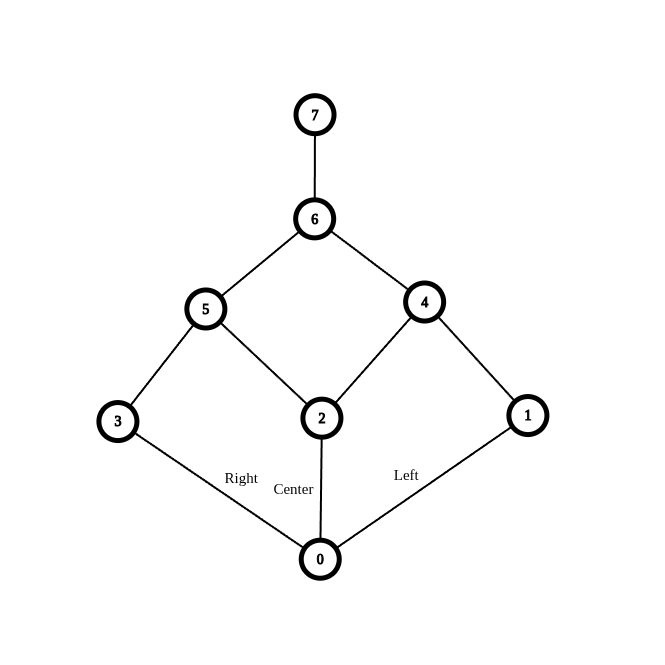
\includegraphics[width=\linewidth]{graph (1).png}
    \end{minipage}\hfill
    \begin{minipage}{0.48\columnwidth}
      \centering
      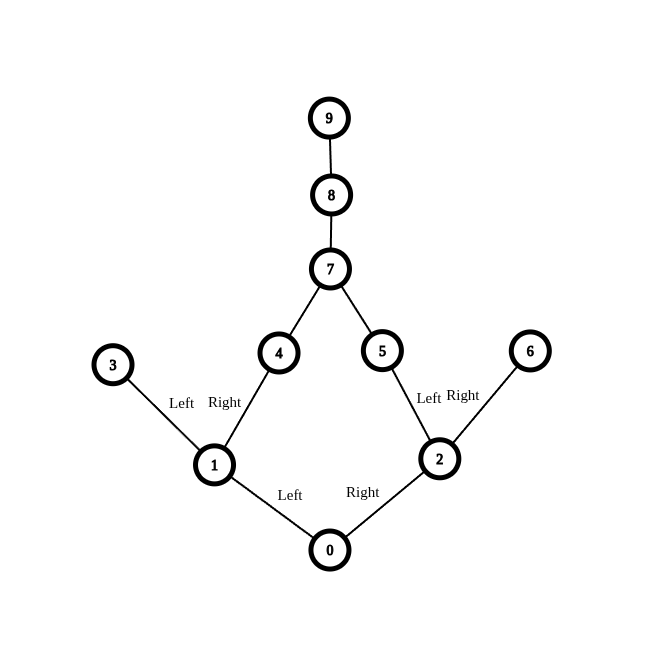
\includegraphics[width=\linewidth]{graph (2).png}
    \end{minipage}
    \caption{Examples of object-support graphs parsed by the VLM from target
    assembly specifications. Directed edges encode direct support relations that are
    later used for branch aggregation and hierarchy-aware batch cutting.}
    \label{fig:layered_graph}
  \end{figure}

  \subsection{Multilevel Graph Partitioning for Branch Aggregation}
  \label{subsec:phase2a}

  A direct topological batching of $\mathcal{G}$ tends to fragment the structure too
  early, because branch discovery and execution ordering become entangled in the same
  local rule set. We instead separate these two tasks. The first task is \emph{branch
  aggregation}: identifying which nodes should be viewed as belonging to the same
  structural branch before any solver-facing batches are emitted.

  To this end, we derive an auxiliary weighted graph
  $\bar{\mathcal{G}}=(\mathcal{V},\bar{\mathcal{E}},W)$ from the directed support graph.
  For branch aggregation, edge orientation is temporarily ignored, but the original
  directed support relation is preserved for the later precedence stage. The edge
  weight $w_{uv}$ encodes structural affinity. Edges inside a single-support chain are
  assigned stronger affinity, whereas edges entering a multi-support transition are
  assigned lower affinity so that structurally merged regions can start a new branch.
  We then solve a multilevel graph partitioning problem \cite{cite_graph_partition_1998}
  to obtain a branch set $\mathcal{P}=\{P_1,\ldots,P_m\}$:
  \begin{equation}
    \min_{\mathcal{P}}
    \sum_{(u,v)\in \bar{\mathcal{E}}}
    w_{uv}\,\mathbb{I}\!\left[\pi(u)\neq\pi(v)\right]
    +
    \lambda \sum_{j=1}^{m}\left||P_j|-\bar{s}\right|,
    \label{eq:partition_objective}
  \end{equation}
  where $\pi(v)$ denotes the partition index of node $v$, $\bar{s}$ is a target
  branch scale, and $\lambda$ balances cut quality against partition size. The
  multilevel procedure follows the standard coarsen-partition-refine pattern: it first
  coarsens the graph, partitions the coarse graph, and then uncoarsens and refines the
  result on progressively finer graphs.

  On the representative support graph used throughout this draft, the aggregation stage
  identifies three branch-level groups: the left support branch $134$, the right
  support branch $256$, and the upper bridge chain $789$. This intermediate result is
  not yet an execution sequence. Its purpose is to recover coherent structural regions
  before we decide how to cut them into solver-facing batches.

  \subsection{Hierarchy-Aware Batch Cutting}
  \label{subsec:phase2b}

  After branch aggregation, each branch subgraph is converted into execution batches
  through hierarchy-aware cutting. This second stage is responsible for the actual
  solver-facing decomposition. It operates on the original directed support graph so
  that every emitted batch remains consistent with precedence.

  For each branch subgraph $P_j$, we recover its induced directed support graph and
  compute a local depth for every node. The branch is then scanned from lower layers to
  higher layers, and nodes are grouped into local batches according to three rules:
  \textit{(i)} every predecessor of a node in the current batch must already have been
  realized, \textit{(ii)} the current batch must remain within the solver scale, and
  \textit{(iii)} nodes from the same local layer are grouped together only when they
  play the same immediate structural role inside the branch. This yields an execution
  sequence that is still grounded in the original hierarchy of the branch rather than
  in an arbitrary topological order.

  In the running example, hierarchy-aware cutting transforms the aggregated branches
  into the local sequences $134 \mapsto 1 \mid 34$, $256 \mapsto 2 \mid 56$, and
  $789 \mapsto 7 \mid 8 \mid 9$. A precedence-consistent ordering over the aggregated
  branch graph then produces the final global execution sequence
  $1 \mid 34 \mid 2 \mid 56 \mid 7 \mid 8 \mid 9$. This two-stage decomposition is
  easier to explain than the previous rule-based batching scheme because branch
  discovery and execution cutting are handled explicitly as different optimization
  problems.

  \subsection{Selective Native LGP Instantiation and Solving}
  \label{subsec:phase3}

  Native LGP couples symbolic task structure with continuous trajectory
  optimization through a shared representation of predicates, action semantics,
  and decision rules~\cite{cite_lgp_2015}. In principle, this abstraction can
  solve assembly tasks from symbolic goals alone. In long-horizon settings,
  however, directly exposing the full generic task domain still leads to
  excessive symbolic branching and unnecessary geometric backtracking.

  Our solver therefore instantiates the native LGP abstraction selectively for
  each execution batch. Once a batch has been determined by the support graph,
  the system reads the scene-order dictionary generated during scene grounding,
  binds generic object categories to concrete scene instances, and compiles only
  the symbolic relations, object bindings, and decision rules required by the
  current support pattern. The solver thus receives a grounded
  symbolic-geometric subproblem tailored to the current batch rather than a
  monolithic domain covering all possible assembly alternatives.

  The same waypoint-level solve also provides geometric cues for downstream
  motion optimization. Let $x$ denote the full-motion trajectory optimized in
  the downstream stage, let $d_{ij}(x)$ denote the minimum pairwise distance
  between robot link $l_i$ and object $o_j$ along $x$, and let $l_i^w$ denote
  the pose of link $l_i$ at waypoint $w$. The downstream trajectory is obtained
  by solving
  \begin{equation}
    x^* = \arg\min_x J(x),
    \label{eq:active_objective}
  \end{equation}
  subject to collision constraints instantiated only for the active set
  \begin{equation}
    c_{ij}(x) = d_{\mathrm{safe}} - d_{ij}(x) \leq 0,
    \quad \forall (l_i, o_j) \in \mathcal{C}_{\mathrm{active}}(w),
    \label{eq:active_constraints}
  \end{equation}
  where
  \begin{equation}
    \mathcal{C}_{\mathrm{active}}(w) =
    \left\{(l_i, o_j)\ \middle|\ d(l_i^w, o_j) < r_{\mathrm{active}}\right\}.
    \label{eq:active_set}
  \end{equation}
  Here, $J(x)$ denotes the downstream motion objective, $d_{\mathrm{safe}}$ is
  the prescribed safety margin, and $r_{\mathrm{active}}$ is the activation
  radius used to screen candidate collision pairs from waypoint geometry.
  Only pairs selected by $\mathcal{C}_{\mathrm{active}}(w)$ are instantiated
  as explicit collision constraints in the downstream full-motion solve. This
  active-constraint strategy reduces unnecessary collision checks and shortens
  full-motion solve time without altering the structural plan itself.

  This restricted instantiation preserves the expressiveness of native LGP while
  concentrating the search on the structurally relevant portion of the task. It
  also provides a clean interface between graph-level decomposition and
  geometric solving: the decomposition module decides which support relations should be
  realized next, and native LGP resolves whether and how those relations can be
  executed under the current scene geometry.

  \subsection{Robot Execution}
  \label{subsec:phase4}

  After each subproblem is solved, the resulting trajectory is parsed and
  dispatched to the robot controller for execution. The execution layer remains
  intentionally thin: it reads the planned motion and gripper commands, executes
  them on the real platform, and updates the scene state for the next
  planning-solving cycle.


  \section{Experimental Results}
  \subsection{Representative Decomposition Case Study}

  We use the representative support graph in
  Figure~\ref{fig:layered_graph} as a running case to clarify the decomposition logic.
  The previous rule-based batching scheme emits the sequence
  $1 \mid 2 \mid 34 \mid 56 \mid 7 \mid 8 \mid 9$. In contrast, the revised method
  first aggregates the graph into the structural groups $134 \mid 256 \mid 789$ and
  only then cuts these groups according to local hierarchy, producing
  $1 \mid 34 \mid 2 \mid 56 \mid 7 \mid 8 \mid 9$. The difference is not merely a
  reordering. The revised method keeps structurally coherent branches intact during the
  aggregation stage and delays fine-grained cutting until the hierarchy of each branch
  has been made explicit.

  \begin{table}[!t]
    \centering
    \caption{Comparison of decomposition strategies on the representative support graph.}
    \label{tab:decomposition_comparison}
    \begin{tabular}{lll}
      \toprule
      Strategy & Branch-level view & Final batch sequence \\
      \midrule
      Previous rule-based batching & not explicit & $1 \mid 2 \mid 34 \mid 56 \mid 7 \mid 8 \mid 9$ \\
      Proposed two-stage decomposition & $134 \mid 256 \mid 789$ & $1 \mid 34 \mid 2 \mid 56 \mid 7 \mid 8 \mid 9$ \\
      \bottomrule
    \end{tabular}
  \end{table}

  \subsection{Evaluation Focus of the Current Draft}

  The current draft focuses on explaining the decomposition logic rather than on
  claiming finalized quantitative gains. The intended evaluation protocol compares the
  previous rule-based batching strategy and the revised two-stage decomposition in
  terms of solver-facing fragmentation, the number of cross-batch support edges, and
  downstream LGP solve behavior. These quantitative results will be reported after the
  final execution pipeline and visual assets have been aligned with the revised method
  description.

  \section{Conclusion}
  This draft reframes VLM-LGP around a clearer decomposition story for long-horizon
  robotic assembly. Instead of using a hand-written rule-based batching scheme, the
  method now separates structural decomposition into two explicit stages: multilevel
  graph partitioning for branch aggregation and hierarchy-aware batch cutting for
  execution ordering. This change makes the interface between support-graph parsing and
  native LGP instantiation easier to explain, easier to analyze, and better aligned
  with the current representative example. Future revisions will extend the
  experimental section with quantitative evidence that compares this revised
  decomposition against the previous rule-based pipeline.

  \begin{thebibliography}{1}
    % --- 核心 LGP 文献 ---

    \bibitem{cite_lgp_2015} M.~Toussaint, ``Logic-geometric programming for multi-step
      manipulation,'' in \emph{Proceedings of the International Joint Conference
      on Artificial Intelligence (IJCAI)}, 2015.

    \bibitem{cite_komo_2014} M.~Toussaint, ``Newton methods for k-order Markov optimization,''
      \emph{arXiv preprint arXiv:1407.0414}, 2014.

    \bibitem{cite_graph_partition_1998} G.~Karypis and V.~Kumar, ``Multilevel
      k-way partitioning scheme for irregular graphs,'' \emph{Journal of Parallel
      and Distributed Computing}, vol.~48, no.~1, pp.~96--129, 1998.

    % --- 改进版 LGP 相关文献 (已收录供后续引用) ---

    \bibitem{cite_rlgp_2023} J.~Schoeler, F.~T.~Rehder, and M.~Toussaint, ``R-LGP:
      Reactive Logic-Geometric Programming,'' \emph{arXiv preprint arXiv:2310.02791},
      2023.

    \bibitem{cite_rhhlgp_2021} J.~Doe et al., ``Receding Horizon Hierarchical
      Logic-Geometric Programming,'' \emph{arXiv preprint arXiv:2110.03420}, 2021.

    \bibitem{cite_text2motion_2023} F.~Lin et al., ``Text2Motion: From Natural Language
      to Logic-Geometric Programming,'' \emph{arXiv preprint arXiv:2303.12153},
      2023.

    \bibitem{cite_vla_placeholder} General VLA Reference, ``Vision-Language-Action
      Models for Robotics,'' \emph{Placeholder}, 2024.

    \bibitem{IEEEhowto:kopka} H.~Kopka and P.~W. Daly, \emph{A Guide to \LaTeX},
      3rd~ed., 1999.

    \bibitem{cite_arxiv_2410_02193} M.~Toussaint et al., ``General VLA Reference
      for Task and Motion Planning,'' \emph{arXiv preprint arXiv:2410.02193}, 2024.

    \bibitem{cite_arxiv_2407_09829} J.~Doe et al., ``Vision-Language Models for
      Robotic Assembly,'' \emph{arXiv preprint arXiv:2407.09829}, 2024.

    \bibitem{cite_arxiv_2506_05168} Y.~Zhu et al., ``Fabrica: Dual-Arm Assembly of
      General Multi-Part Objects via Integrated Planning and Learning,'' \emph{arXiv
      preprint arXiv:2506.05168}, 2024.

    % --- 经典 TAMP/PDDL 文献 ---

    \bibitem{cite_pddl_1998} D.~McDermott \emph{et al.}, ``PDDL-the planning
      domain definition language,'' \emph{Technical Report, Yale Center for Computational
      Vision and Control}, 1998.
  \end{thebibliography}
\end{document}
